\begin{figure}[!bt]
  \begin{center}
    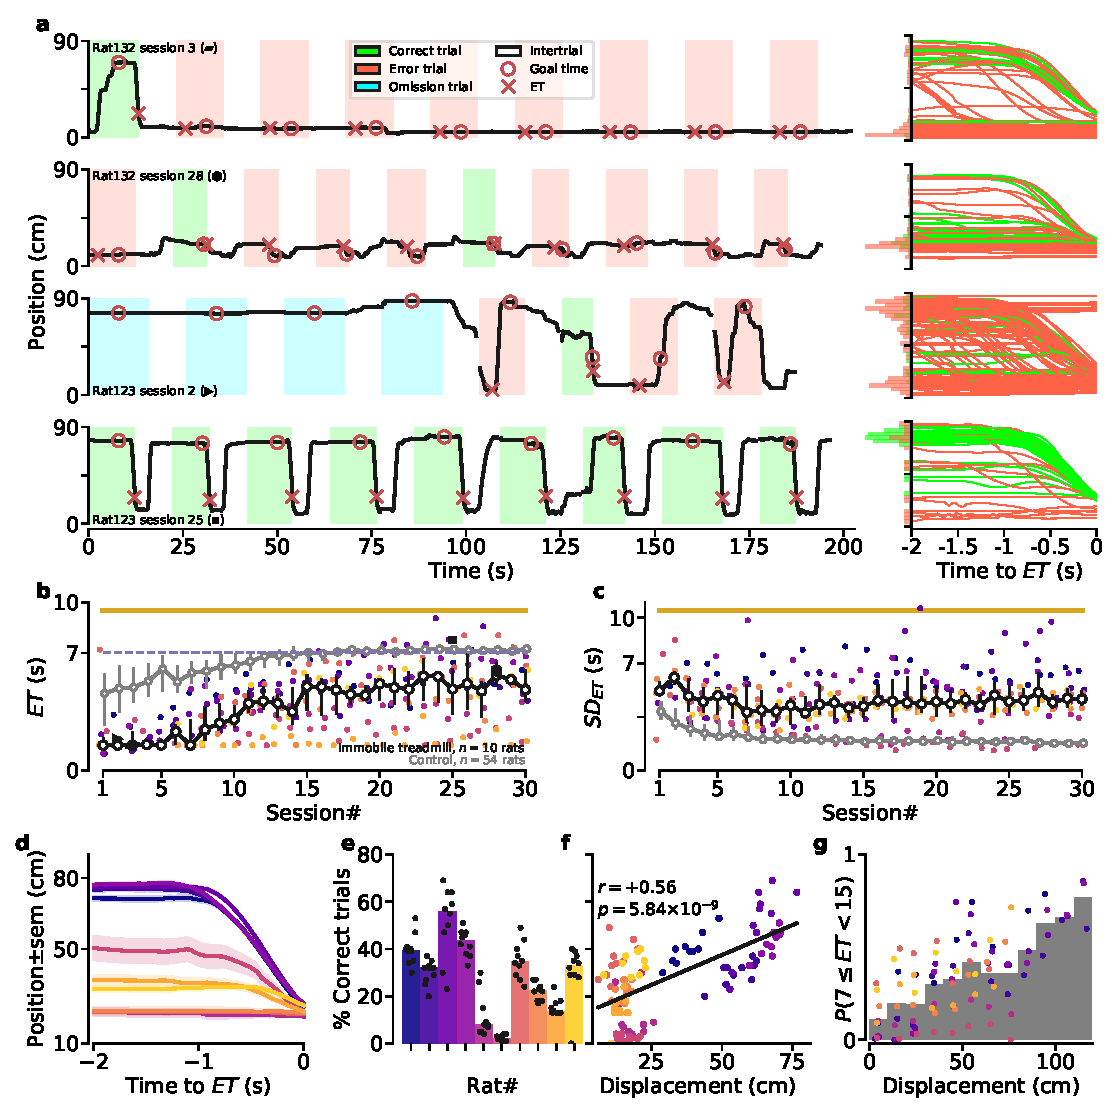
\includegraphics[width=.8\linewidth]{ch-time/figures/ImmTrd.pdf}
    \caption[Immobile Condition]
    {\textbf{Performance of animals trained while the treadmill remained immobile.}
    \textbf{a)}
    \textit{Left}: illustrations of the positions of two animals on the immobile treadmill for 9~consecutive trials, early (\textit{1st row:}~Rat~\#132-session~\#3, \textit{3rd row:} Rat~\#123-session~\#2) and late (\textit{2nd row:} Rat~\#132-session~\#28, \textit{4th row:} Rat~\#123-session~\#25) during training.
    \textit{Right}: trajectories for all the trials of the corresponding sessions on the left, aligned to the $ET$.
    Distributions of positions 2~s before $ET$, for correct (green) and error (red) trials are shown on the y-axis.
    \textbf{b)}
    Median $ET$ across sessions for ``immobile treadmill'' animals.
    Filled black markers correspond to the sessions illustrated in panel~a.
    Horizontal line indicates significant group difference (permutation test).
    \textbf{c)}
    Similar to panel~b, for the standard deviation of entrance times ($SD_{ET}$).
    \textbf{d)}
    Median trajectory aligned to $ET$ of each immobile treadmill animal (only correct trials from sessions~\#20 to~\#30 are considered; shaded area denotes standard error).
    \textbf{e)}
    Median percentage of correct trials for each immobile treadmill animal.
    Each dot represents one session.
    \textbf{f)}
    Repeated measures correlation between the percentage of correct trials and average displacement during a session.
    Each dot represents one session.
    \textbf{g)}
    PDF of a correct trial, given the displacement of an animal.
    Each dot represents the average probability for an individual animal, during a single session.
    \textbf{(e-g)}
    Analyses include the same sessions as in panel~d.
    Individual animal color code is preserved in panels~b-g.
    }
    \label{fig:time:ImmTrd}
  \end{center}
\end{figure}